\documentclass[final,hyperref={pdfpagelabels=false}]{beamer}
\mode<presentation>
\usepackage{color}
\usepackage[size=custom,width=36,height=48,scale=.8,orientation=portrait]{beamerposter}
\usepackage{tikz}
\usepackage{tikzscale}

\setbeamertemplate{navigation symbols}{}
\usetheme[poster]{memsys}

\title{Portable Application Guidance for Complex Memory Systems}
\author{M. Ben Olson, Brandon Kammerdiener, Michael R. Jantz, Kshitij A. Doshi, Terry Jones}

\begin{document}
\begin{frame}{}
\begin{columns}[t]
  \begin{column}{.45\linewidth}

    % Problem
    \begin{block}{Problem}
      \begin{columns}%
        \column{.46\textwidth}%
        \includegraphics[width=1\textwidth]{tikz/tiers.tikz}
        \column{.45\textwidth}%
        Memory is no longer a contiguous block of
        volatile DRAM with homogeneous performance.
      \end{columns}%
      \vspace{1mm}%
    \end{block}

    \begin{block}{Current Approaches}
      \begin{itemize}
				\item \highlight{Cache Mode}:
          Upper tier as hardware-managed cache (Cache Mode on KNL, 2LM on CLX).
          Inflexible and subject to nasty edge cases.
				\item \highlight{First touch}:
					Software-based data tiering (\texttt{numactl}). Produces inconsistent, often poor,
          performance.
      \end{itemize}
    \end{block}

    \begin{block}{Our Approach}
      We use automated compile-time annotation, PEBS-based profiling, and arena
      allocation to collect per-allocation-site memory usage and intelligently
      guide and migrate data placement.
      \vspace{1em}
      \begin{center}
        \resizebox{0.85\textwidth}{!}{%
          \begin{tikzpicture}[>={LaTeX[width=5mm]},->,
                    line width=1mm,
                    shorten >=0.3cm]


  \ifposter
    \huge
    \newcommand\WIDTH{150mm}
    \newcommand\HEIGHT{120mm}
    \newcommand\TITLEHEIGHT{25mm}
    \newcommand\BODYHEIGHT{95mm}
    \newcommand\OFFSET{20mm}
  \else
    \ifpres
      \giant
      \newcommand\WIDTH{200mm}
      \newcommand\HEIGHT{200mm}
    \fi
  \fi

  % Styles
  \tikzstyle{bigbox} = [draw,
                        rectangle,
                        minimum width=\WIDTH,
                        minimum height=\HEIGHT,
                        align=center,
                        inner sep=5mm,
                        outer sep=0mm]
  \tikzstyle{title} = [draw,
                        rectangle,
                        minimum width=\WIDTH,
                        minimum height=\TITLEHEIGHT,
                        align=center,
                        inner sep=5mm,
                        outer sep=0mm]
  \tikzstyle{body} = [draw,
                        rectangle,
                        minimum width=\WIDTH,
                        minimum height=\BODYHEIGHT,
                        align=center,
                        inner sep=5mm,
                        outer sep=0mm]

  % Annotate
  \node[bigbox](annotate){};
  \node[title, below=0mm of annotate.north](annotatetitle){
    \highlight{Annotate}
  };
  \node[body, below=0mm of annotatetitle](annotatebody){
    Compile executable\\with allocation site\\annotations
  };

  % Profile
  \node[bigbox, below=\OFFSET of annotate.south](profile){};
  \node[title, below=0mm of profile.north](profiletitle){
    \highlight{Profile}
  };
  \node[body, below=0mm of profiletitle](profilebody){
    Profile memory\\usage of each site
  };

  % Decide
  \node[bigbox, right=0.75*\WIDTH of annotate.east](decide){};
  \node[title, below=0mm of decide.north](decidetitle){
    \highlight{Decide}
  };
  \node[body, below=0mm of decidetitle](decidebody){
    Generate tier\\recommendations
  };

  % Apply
  \node[bigbox, below=\OFFSET of decide.south](apply){};
  \node[title, below=0mm of apply.north](applytitle){
    \highlight{Apply}
  };
  \node[body, below=0mm of applytitle](applybody){
    Bind memory\\according to tier\\recommendations
  };

  \path[] (annotate.south) edge[] node {} (profile.north);
  \path[] (profile.east) edge[] node {} (decide.west);
  \path[] (decide.south) edge[] node {} (apply.north);

\end{tikzpicture}

        }
      \end{center}
    \end{block}

    % Try It Out
    \begin{block}{Try It Out}
        https://github.com/lanl/SICM/tree/high\_dev
        \\\vspace{1em}
        Currently it's a branch of the main SICM repository. We plan to merge when it stabilizes.
    \end{block}


  \end{column}
  
  \begin{column}{.45\linewidth}

    % Solution
    \begin{block}{Framework}
      \highlight{SICM}:\\Simplified Interface to Complex Memory
      \begin{center}
        \resizebox{0.7\textwidth}{!}{%
          \begin{tikzpicture}[>={LaTeX[width=5mm]},->,
                    line width=1mm,
                    shorten >=0.3cm]

  \ifposter
    \quitebig
    \newcommand\WIDTH{120mm}
    \newcommand\HEIGHT{138mm}
    \newcommand\BOXHEIGHT{90mm}
    \newcommand\INNERBOXSEP{-10mm}
    \newcommand\OUTERBOXSEP{6mm}
    \newcommand\BIGSPACER{95mm}
    \newcommand\SMALLSPACER{40mm}
  \else
    \ifpres
      \giant
      \newcommand\WIDTH{170mm}
      \newcommand\HEIGHT{190mm}
      \newcommand\BOXHEIGHT{100mm}
      \newcommand\INNERBOXSEP{-20mm}
      \newcommand\OUTERBOXSEP{8mm}
      \newcommand\BIGSPACER{140mm}
      \newcommand\SMALLSPACER{59mm}
    \fi
  \fi

  % Styles
  \tikzstyle{bigbox} = [draw, 
                        rectangle,
                        minimum width=4.5*\WIDTH,
                        minimum height=\HEIGHT,
                        align=center,
                        inner sep=0mm,
                        outer sep=0mm]
  \tikzstyle{box} = [draw, 
                     regular polygon,
                     regular polygon sides=5,
                     anchor=center,
                     outer sep=\OUTERBOXSEP,
                     inner sep=\INNERBOXSEP,
                     minimum width=\WIDTH,
                     minimum height=\BOXHEIGHT,
                     align=center]
  \tikzstyle{halfbox} = [
                     rectangle,
                     anchor=center,
                     outer sep=0mm,
                     inner sep=0mm,
                     yshift=-20mm,
                     minimum width=\BIGSPACER,
                     minimum height=1mm,
                     align=center]
  \tikzstyle{tinybox} = [
                     rectangle,
                     anchor=center,
                     outer sep=0mm,
                     inner sep=0mm,
                     yshift=-20mm,
                     minimum width=\SMALLSPACER,
                     minimum height=1mm,
                     align=center]

  \node[bigbox](a){};
  \node[tinybox, right=0pt of a.west](a0){};
  \node[box, right=0pt of a0.east](a1){\highlight{A}\\Compiler\\Wrappers};
  \node[box, right=0pt of a1.east](a2){\highlight{B}\\Profiling};
  \node[box, right=0pt of a2.east](a3){\highlight{C}\\Placement\\Algorithms};
  \node[box, right=0pt of a3.east](a4){\highlight{D}\\Smart\\Allocation};
  \node[tinybox, right=0pt of a4.east](a5){};
  \node[align=center, below=0pt of a.north](title0){\highlight{High-Level Interface}};

  \node[bigbox, below=0pt of a](b){};
  \node[tinybox, right=0pt of b.west](b0){};
  \node[box, right=0pt of b0.east](b1){Discovery};
  \node[box, right=0pt of b1.east](b2){Config};
  \node[box, right=0pt of b2.east](b3){Allocation};
  \node[box, right=0pt of b3.east](b4){Arena\\Allocation};
  \node[tinybox, right=0pt of b4.east](b5){};
  \node[align=center, below=0pt of b.north](title1){\highlight{Low-Level Interface}};

  \node[bigbox, below=0pt of b](c){};
  \node[halfbox, right=0pt of c.west](c0){};
  \node[box, right=0pt of c0.east](c1){NUMA\\API};
  \node[box, right=0pt of c1.east](c2){\texttt{mbind}};
  \node[box, right=0pt of c2.east](c3){\texttt{madvise}};
  \node[halfbox, right=0pt of c3.east](c4){};
  \node[align=center, below=0pt of c.north](title2){\highlight{Kernel}};

  \node[bigbox, below=0pt of c](d){};
  \node[halfbox, right=0pt of d.west](d0){};
  \node[box, right=0pt of d0.east](d1){MCDRAM};
  \node[box, right=0pt of d1.east](d2){DCPMMs};
  \node[box, right=0pt of d2.east](d3){DRAM};
  \node[halfbox, right=0pt of d3.east](d4){};
  \node[align=center, below=0pt of d.north](title3){\highlight{Devices}};

\end{tikzpicture}

        }%
      \end{center}%
    \end{block}

    % Results
    \begin{block}{Results}
      \centering%
      \highlight{Varying Capacity:}\\
      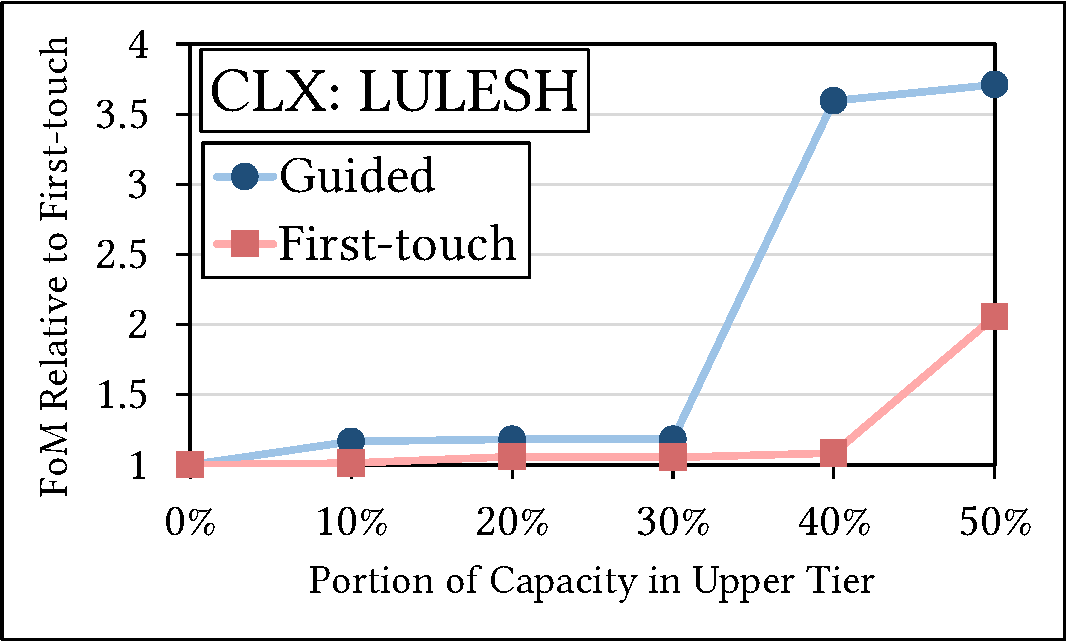
\includegraphics[width=0.45\textwidth]{figures/clx_small_lulesh.pdf}
      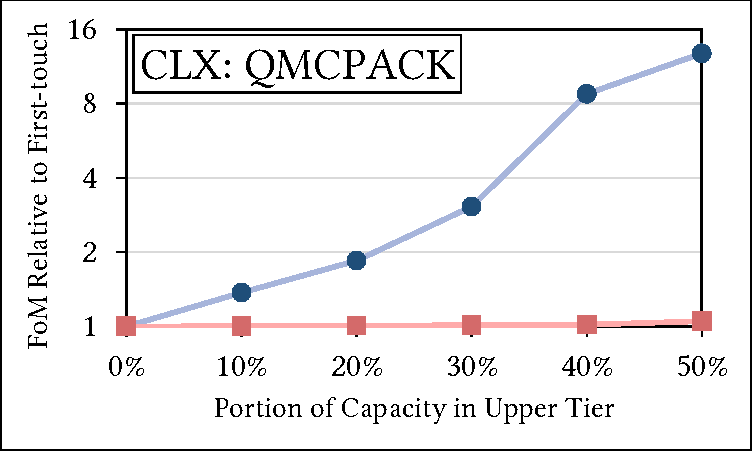
\includegraphics[width=0.45\textwidth]{figures/clx_small_qmcpack.pdf}
      \highlight{KNL Performance:}
      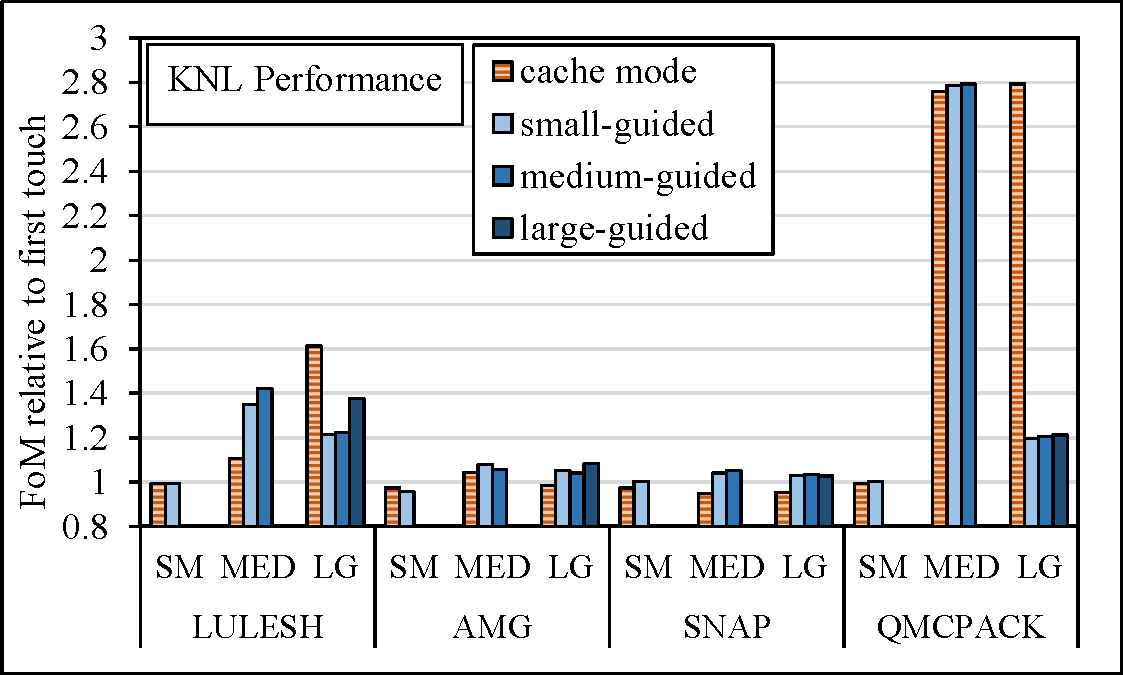
\includegraphics[width=0.8\textwidth]{figures/knl_perf.pdf}\\
      \vspace{1em}
      \highlight{CLX Performance:}
      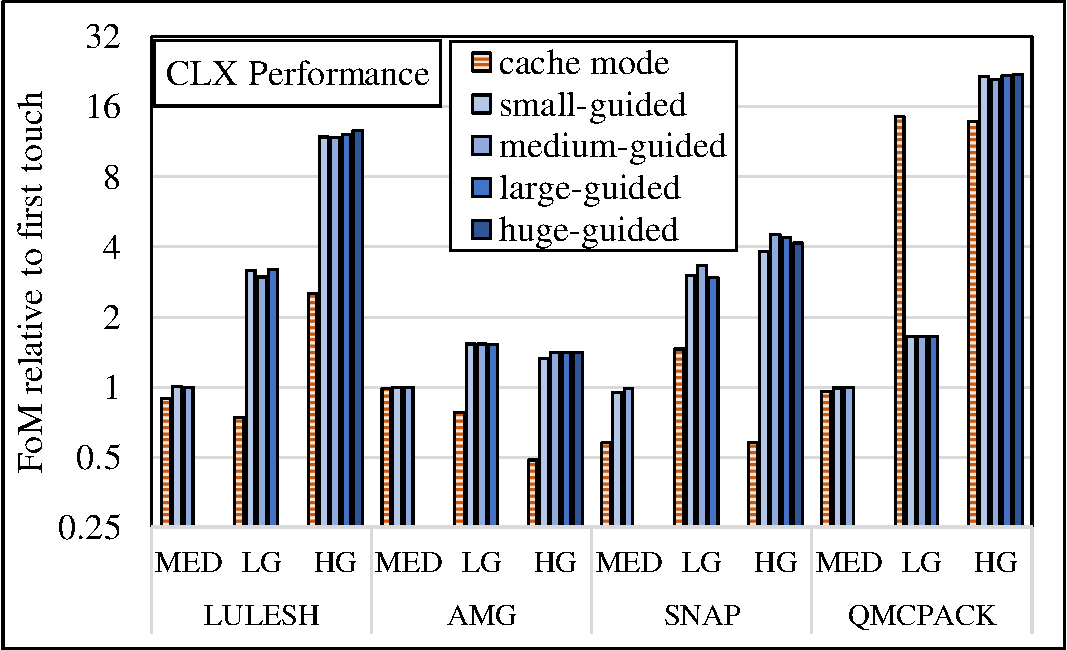
\includegraphics[width=0.8\textwidth]{figures/aep_perf.pdf}\\
    \end{block}

  \end{column}
\end{columns}
\end{frame}
\end{document}
